\section{Results}
\label{resultSection}
\subsection{Compute Resource Utilization}
While the performance testing is focused on comparing the overall Istio system resource utilization of sidecar and ambient modes, a quick look at one of the microservice pod resource consumptions in both modes is a good starting point.

\begin{figure}[ht!]
  \centering
  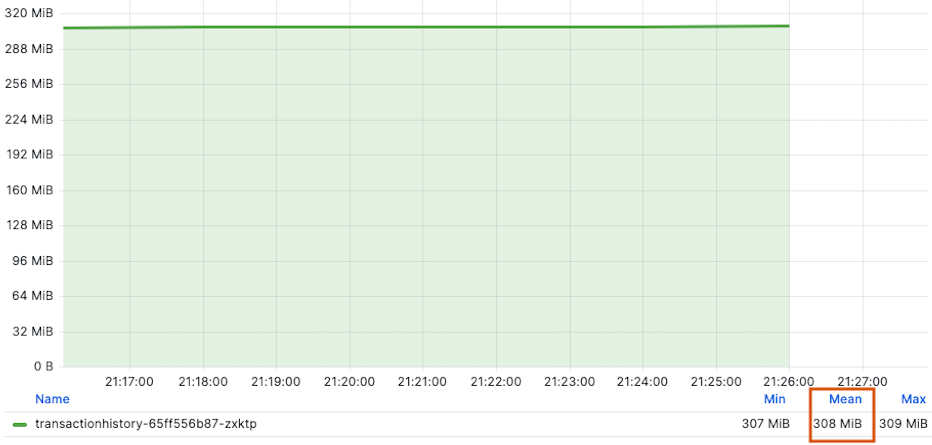
\includegraphics[width=0.85\linewidth]{resources/sidecar-pod-mem.png}
  \caption{Pod Memory Use in Sidecar Mode}
  \label{result:podMemUseSidecar}
\end{figure}

\begin{figure}[ht!]
  \centering
  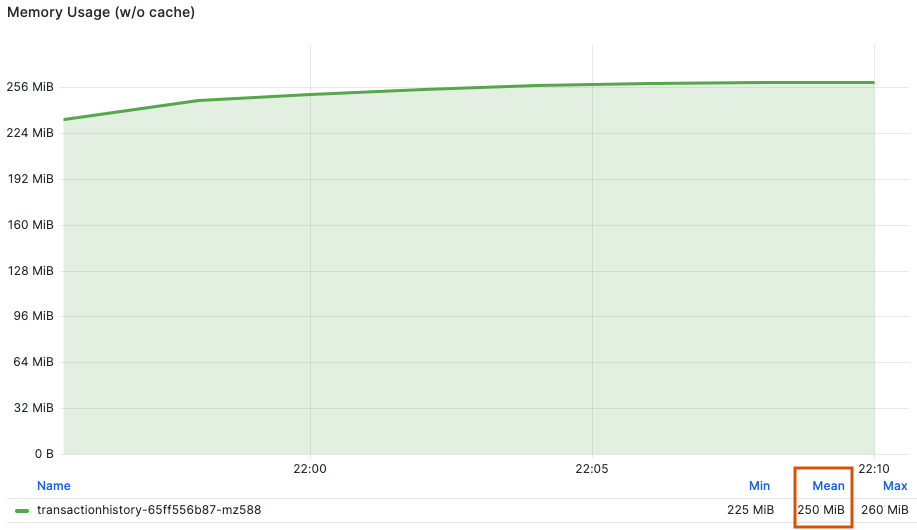
\includegraphics[width=0.85\linewidth]{resources/ambient-pod-mem.png}
  \caption{Pod Memory Use in Ambient Mode}
  \label{result:podMemUseAmbient}
\end{figure}

Figure \ref{result:podMemUseSidecar} and \ref{result:podMemUseAmbient} shows a ten minutes memory usage graph of transaction history microservice pod in sidecar and ambient mode. In sidecar mode the average memory usage reported is 308\gls{mib} whereas in ambient mode its only 250\gls{mib}. This result interprets an improvement of 23.2\% memory usage in ambient mode however there is no CPU resource utilization difference is noticed.

% \subsubsection{Istio System Resource Utilization}
Section \ref{testReadiness} describes how Istio system resource utilization comparison test is designed with two different environments. As part of the tests across single and multiple namespace deployment, test data is captured from Grafana. In this section test result graphs are shown with a minimum, maximum and a mean value for CPU and memory usage over a ten minutes time period. All the test result graphs can be intimidating hence before jumping into those, Table  and  briefs the results in a tabular form.

% \begin{table}[ht!]
%   \centering
%   \begin{tabular}{ |l|c|c|c|}
%     \hline
%     \textbf{Test Environment} & \textbf{\textit{Min}} & \textbf{\textit{Mean}} & \textbf{\textit{Max}} \\ \hline
%     Single Namespace & 584 & 67.3 & 120 \\ \hline
%     Multiple Namespaces & 1843.2 & 88.6 & 461 \\ \hline 
%   \end{tabular}
%   \caption{Different \textit{memory} Usage in MiB}
%   \label{allCpuResultsTable}
% \end{table}

% \begin{table}[ht!]
%   \centering
%   \begin{tabular}{ |l|c|c|c|}
%     \hline
%     \textbf{Test Environment} & \textbf{\textit{Sidecar}} & \textbf{Ambient L4} & \textbf{Ambient L4 + L7} \\ \hline
%     Single Namespace & 584 & 67.3 & 120 \\ \hline
%     Multiple Namespaces & 1843.2 & 88.6 & 461 \\ \hline 
%   \end{tabular}
%   \caption{Comparison \textit{memory} values in MiB}
%   \label{allMemResultsTable}
% \end{table}


%%single ns
%sidecar cpu, mem
\begin{figure}[H]
  \centering
  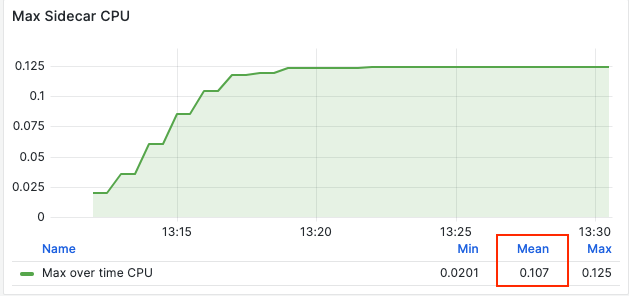
\includegraphics[width=0.8\linewidth]{resources/max-sidecar-cpu.png}
  \caption{CPU Usage of Sidecar Mode in Single Namespace}
\end{figure}

\begin{figure}[H]
  \centering
  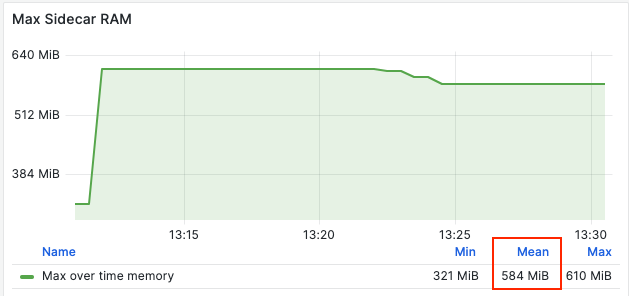
\includegraphics[width=0.8\linewidth]{resources/max-sidecar-mem.png}
  \caption{Memory Usage of Sidecar Mode in Single Namespace}
\end{figure}

%ambient l4 cpu, mem
\begin{figure}[H]
  \centering
  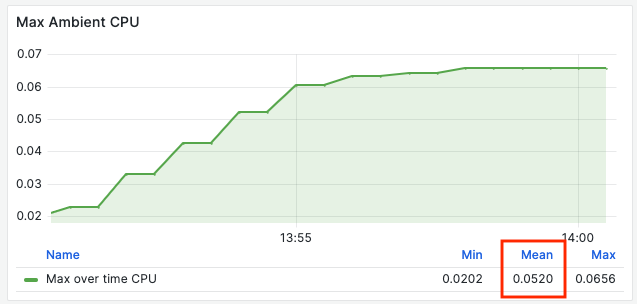
\includegraphics[width=0.8\linewidth]{resources/max-ambient-l4-cpu.png}
  \caption{CPU Usage of Ambient Mode(L4 Only) in Single Namespace}
\end{figure}

\begin{figure}[H]
  \centering
  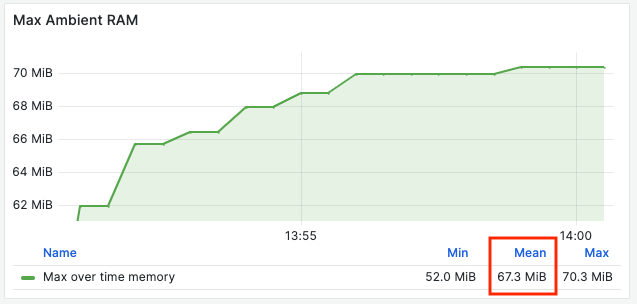
\includegraphics[width=0.8\linewidth]{resources/max-ambient-l4-mem.png}
  \caption{Memory Usage of Ambient Mode(L4 Only) in Single Namespace}
\end{figure}

%ambient l4+l7 cpu, mem
\begin{figure}[H]
  \centering
  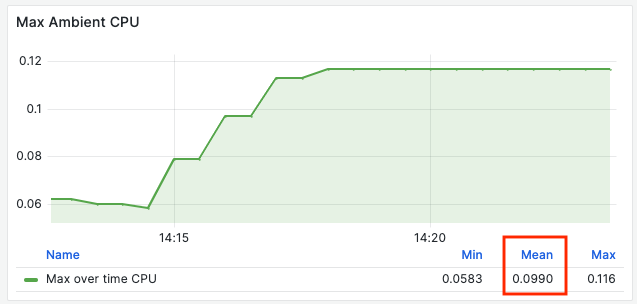
\includegraphics[width=0.78\linewidth]{resources/max-ambient-l4-l7-cpu.png}
  \caption{CPU Usage of Ambient Mode(L4 + L7) in Single Namespace}
\end{figure}

\begin{figure}[H]
  \centering
  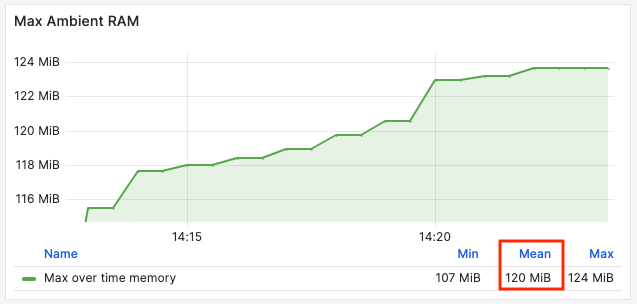
\includegraphics[width=0.8\linewidth]{resources/max-ambient-l4-l7-mem.png}
  \caption{Memory Usage of Ambient Mode(L4 + L7) in Single Namespace}
\end{figure}


%%multi ns
%sidecar cpu, mem
\begin{figure}[H]
  \centering
  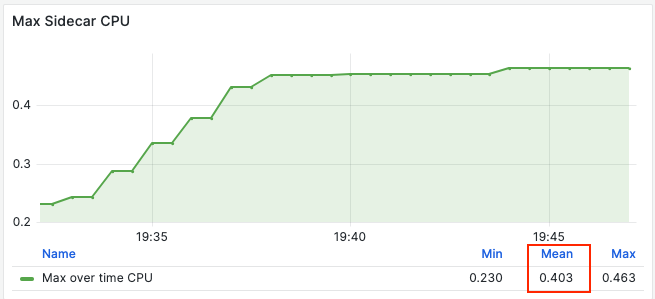
\includegraphics[width=0.8\linewidth]{resources/multi-ns-sidecar-cpu.png}
  \caption{CPU Usage of Sidecar Mode in Multiple Namespace}
\end{figure}

\begin{figure}[H]
  \centering
  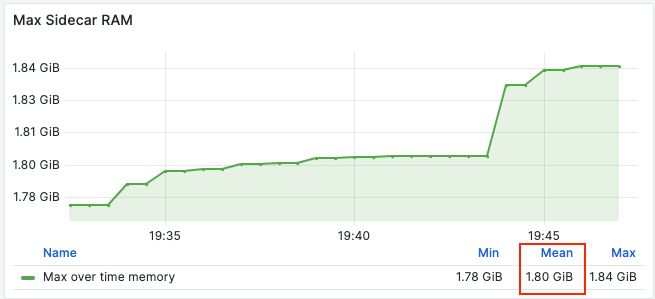
\includegraphics[width=0.8\linewidth]{resources/multi-ns-sidecar-mem.png}
  \caption{Memory Usage of Sidecar Mode in Multiple Namespace}
\end{figure}

%ambient l4 cpu, mem
\begin{figure}[H]
  \centering
  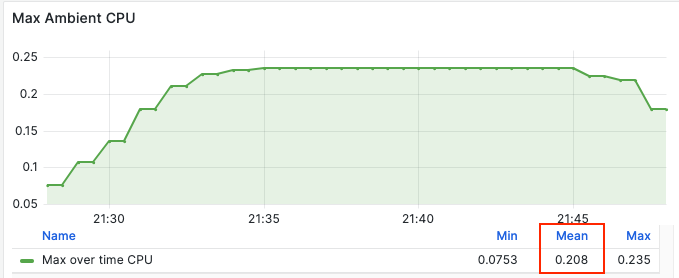
\includegraphics[width=0.8\linewidth]{resources/ambient-multi-ns-l4-cpu.png}
  \caption{CPU Usage of Ambient Mode(L4 Only) in Multiple Namespace}
\end{figure}

\begin{figure}[H]
  \centering
  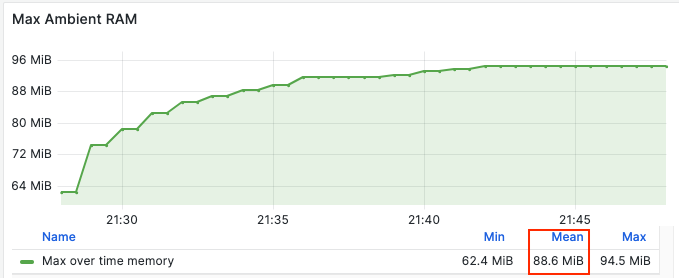
\includegraphics[width=0.85\linewidth]{resources/ambient-multi-ns-l4-mem.png}
  \caption{Memory Usage of Ambient Mode(L4 Only) in Multiple Namespace}
\end{figure}

%ambient l4+l7 cpu, mem
\begin{figure}[H]
  \centering
  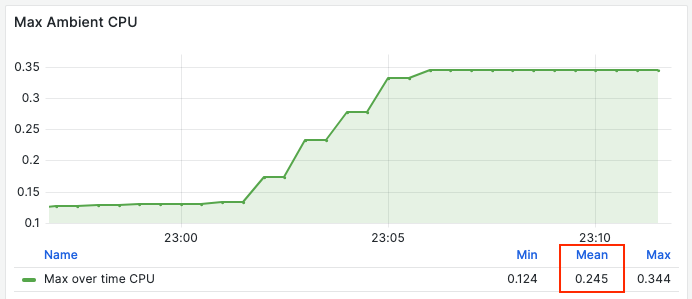
\includegraphics[width=0.85\linewidth]{resources/ambient-multi-ns-l4-l7-cpu.png}
  \caption{CPU Usage of Ambient Mode(L4 + L7) in Multiple Namespace}
\end{figure}

\begin{figure}[H]
  \centering
  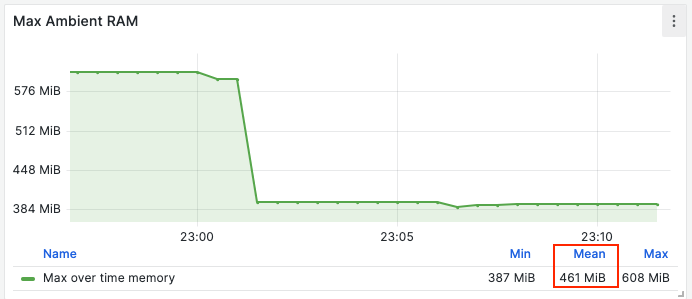
\includegraphics[width=0.85\linewidth]{resources/ambient-multi-ns-l4-l7-mem.png}
  \caption{Memory Usage of Ambient Mode(L4 + L7) in Multiple Namespace}
\end{figure}

With the above test results in place, lets find out the exact performance benefit pecentage by comparing mean values of CPU and memory usage between sidecar mode, ambient mode with L4 proxy and ambient mode with L4 and L7 proxy enabled. Table \ref{cpuUsageTable} shows the CPU utilization of single namespace scenario as 0.1 vCPU for sidecar mode and 0.05 vCPU, 0.09 vCPU in case of ambient L4 only and L4, L7 modes respectively. In multiple namespaces test scenario the numbers changes to 0.40 vCPU for sidecar and 0.20 vCPU, 0.24 vCPU for ambient L4 and L4, L7 mode respectively.

\begin{table}[ht!]
  \centering
  \begin{tabular}{ |l|c|c|c|}
    \hline
    \textbf{Test Environment} & \textbf{\textit{Sidecar}} & \textbf{\textit{Ambient L4}} & \textbf{\textit{Ambient L4+L7}} \\ \hline
    Single Namespace & 0.107 & 0.052 (51.4\%) & 0.099 (7.4\%) \\ \hline
    Multiple Namespaces & 0.403 & 0.208 (48\%) & 0.245 (39\%) \\ \hline
  \end{tabular}
  \caption{CPU Usage in \textit{vCPU} with Improvement \textit{Percentage}}
  \label{cpuUsageTable}
\end{table}

Table \ref{memoryUsageTable} shows the memory utilization in single namespace environment as 584 MiB in sidecar mode whereas in ambient mode with L4 processing 67.3 MiB and with both L4, L7 processing it is 120 MiB. In multiple namespace scenario, the number changes to 1.80 GiB in sidecar mode whereas only 88.6 MiB in ambient L4 mode and 461 MiB when both L4, L7 layers are engaged in ambient mode.

\begin{table}[ht!]
  \centering
  \begin{tabular}{ |l|c|c|c| }
    \hline
    \textbf{Test Environment} & \textbf{\textit{Sidecar}} & \textbf{\textit{Ambient L4}} & \textbf{\textit{Ambient L4+L7}} \\ \hline
    Single Namespace & 584 & 67.3 (88.47\%) & 120 (79.45\%) \\ \hline
    Multiple Namespaces & 1843.2  & 88.6 (95.13\%) & 461 (74.98\%) \\ \hline
  \end{tabular}
  \caption{Memory Usage in \textit{MiB} with Improvement \textit{Percentage}}
  \label{memoryUsageTable}
\end{table}


\subsection{Operational Complexity}
[TBD]
